\chapter{WSTĘP I CEL PRACY}
\label{chap:introduction}
Wstępu wstępu - tutaj należy pokrótce opisać o co chodzi w pracy i wyraźnie wskazać cel pracy!

Wstęp i cel pracy nakreśla problematykę opisaną lub rozwiązywaną w pracy dyplomowej wraz z uzasadnieniem celowości jej realizacji. Podaje cel i ewentualnie tezę (hipotezę). Syntetycznie opisuje dotychczasowe dokonania w danej tematyce, założenia techniczne oraz może zwięźle przedstawić zawartość poszczególnych rozdziałów. W przypadku pracy realizowanej przez kilku studentów, przy omawianiu zawartości rozdziałów należy podać ich autorów. Punkty stanowiące element składowy podrozdziału powinny być opracowane przez jednego autora

% \begin{figure}[H]
%     \centering
%     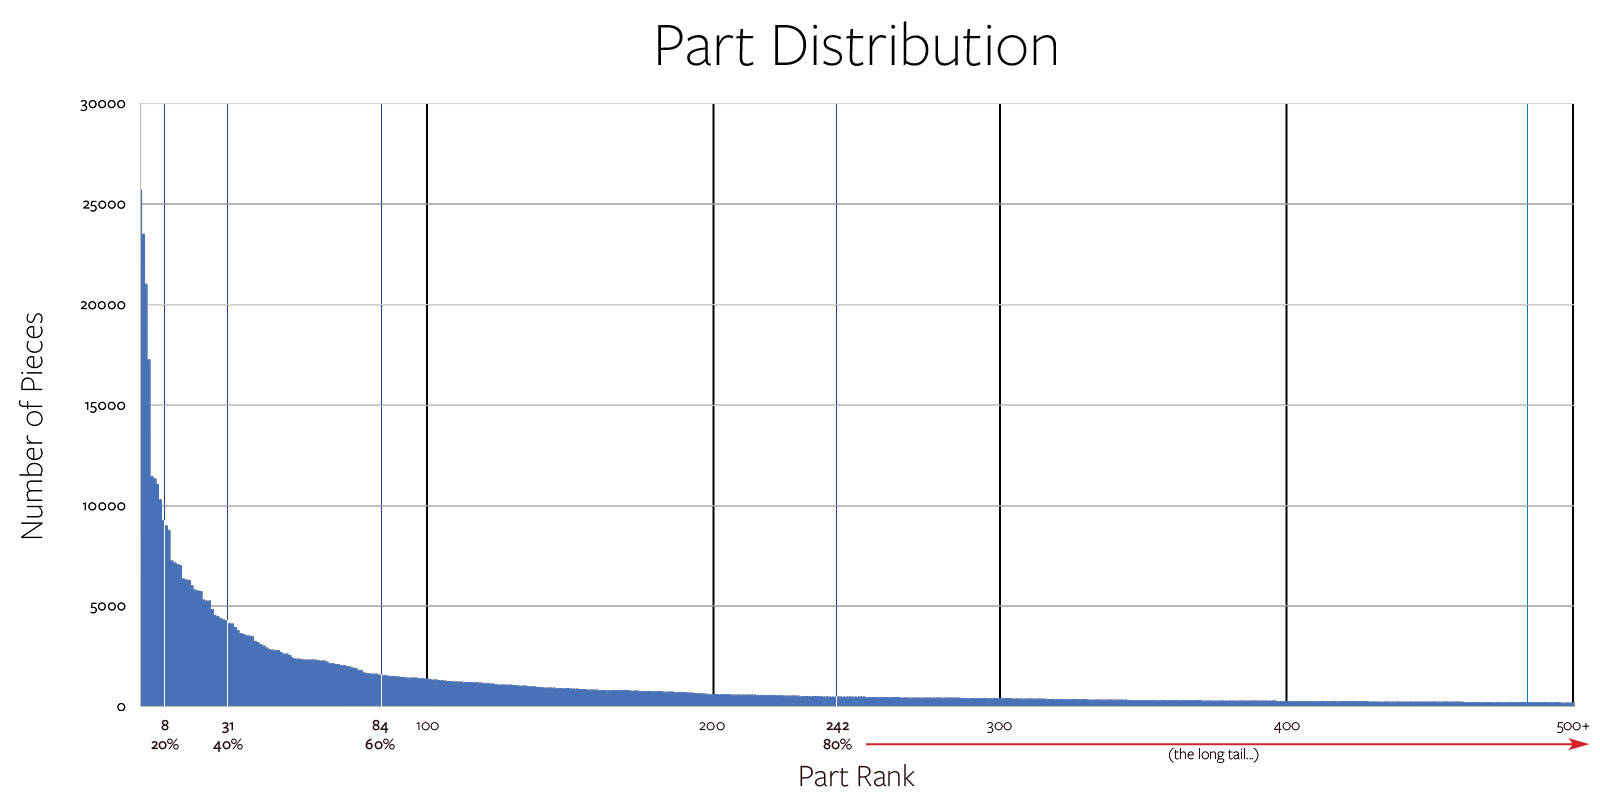
\includegraphics[width=1\textwidth]{images/part_dist.jpg}
%     \caption{Szacunkowa dystrybucja klas klocków kupionych w latach 2015-2020\cite{dist}}
%     \label{fig:part_dist}
% \end{figure}
% Na wykresie \ref{fig:part_dist} terefere.
\section{Cel pracy}
Mój super cel. 
\section{Układ pracy}
Układ pracy jest następujący...

\begin{figure}[htbp]
    \centering
    
\includegraphics[width=0.9\textwidth]{images/obrazek.png}
    \caption{Opis obrazka}
    \label{fig:buzka}
\end{figure}


\begin{table}[h]
\caption{Opis tabelki}
\label{tab:tab1}
 \centering
\begin{tabular}{|c|p{4.5cm}|p{6cm}|}
  \hline
  Pole 1 & Pole 2 & Pole 3\\
  \hline
  1 & Pojęcie & Opis tegoż pojęcia\\
  \hline
  2 & Pojęcie & Opis tegoż pojęcia\\
  \hline
\end{tabular}
% \vspace{-0.5cm}
\end{table}